\section{Experiment}

\subsection{Measurements of the spectral characteristics of the photocell photocurrent}

In this exercise we are going to take measurements of the spectral characteristics of the
photocell photocurrent.



\begin{table}[H]
    \centering
    \begin{tabular}{l|l|l|l|l|l|l|l|l}
    
        $\lambda \SI{}{\nano\meter}$ & $u_{\lambda} \SI{}{\nano\meter}$ & I \SI{}{\micro\ampere} & $u_I$ \SI{}{\micro\ampere}& ~ & $\lambda \SI{}{\nano\meter}$ & $u_{\lambda} \SI{}{\nano\meter}$ & I \SI{}{\micro\ampere} & $u_I$ \SI{}{\micro\ampere} \\ \hline
        370 & 1.2 & 0.2 & 0.116 && 540 & 1.2 & 3.5 & 0.119 \\ \hline
        375 & 1.2 & 0.3 & 0.116 && 545 & 1.2 & 3.3 & 0.119 \\ \hline
        380 & 1.2 & 0.3 & 0.116 && 550 & 1.2 & 3.2 & 0.119 \\ \hline
        385 & 1.2 & 0.4 & 0.116 && 555 & 1.2 & 2.9 & 0.118 \\ \hline
        390 & 1.2 & 0.5 & 0.116 && 560 & 1.2 & 2.8 & 0.118 \\ \hline
        395 & 1.2 & 0.7 & 0.117 && 565 & 1.2 & 2.6 & 0.118 \\ \hline
        400 & 1.2 & 0.8 & 0.117 && 570 & 1.2 & 2.3 & 0.118 \\ \hline
        405 & 1.2 & 0.9 & 0.117 && 575 & 1.2 & 2.1 & 0.118 \\ \hline
        410 & 1.2 & 1 & 0.117 && 580 & 1.2 & 1.9 & 0.118 \\ \hline
        415 & 1.2 & 1.1 & 0.117 && 585 & 1.2 & 1.7 & 0.117 \\ \hline
        420 & 1.2 & 1.3 & 0.117 && 590 & 1.2 & 1.3 & 0.117 \\ \hline
        425 & 1.2 & 1.4 & 0.117 && 595 & 1.2 & 1 & 0.117 \\ \hline
        430 & 1.2 & 1.5 & 0.117 && 600 & 1.2 & 0.7 & 0.117 \\ \hline
        435 & 1.2 & 1.7 & 0.117 && 605 & 1.2 & 0.5 & 0.116 \\ \hline
        440 & 1.2 & 1.9 & 0.118 && 610 & 1.2 & 0.3 & 0.116 \\ \hline
        445 & 1.2 & 2 & 0.118 && 615 & 1.2 & 0.2 & 0.116 \\ \hline
        450 & 1.2 & 2.1 & 0.118 && 620 & 1.2 & 0.2 & 0.116 \\ \hline
        455 & 1.2 & 2.3 & 0.118 && 625 & 1.2 & 0.1 & 0.116 \\ \hline
        460 & 1.2 & 2.4 & 0.118 && 630 & 1.2 & 0.1 & 0.116 \\ \hline
        465 & 1.2 & 2.7 & 0.118 && 635 & 1.2 & 0 & 0.116 \\ \hline
        470 & 1.2 & 2.8 & 0.118 && 640 & 1.2 & 0 & 0.116 \\ \hline
        475 & 1.2 & 3.1 & 0.119 && 645 & 1.2 & 0 & 0.116 \\ \hline
        480 & 1.2 & 3.3 & 0.119 && 650 & 1.2 & 0 & 0.116 \\ \hline
        485 & 1.2 & 3.4 & 0.119 && 655 & 1.2 & 0 & 0.116 \\ \hline
        490 & 1.2 & 3.5 & 0.119 && 660 & 1.2 & 0 & 0.116 \\ \hline
        495 & 1.2 & 3.7 & 0.119 && 665 & 1.2 & 0 & 0.116 \\ \hline
        500 & 1.2 & 3.8 & 0.119 && 670 & 1.2 & 0 & 0.116 \\ \hline
        505 & 1.2 & 3.9 & 0.119 && 675 & 1.2 & 0 & 0.116 \\ \hline
        510 & 1.2 & 3.9 & 0.119 && 680 & 1.2 & 0 & 0.116 \\ \hline
        515 & 1.2 & 3.9 & 0.119 && 685 & 1.2 & 0 & 0.116 \\ \hline
        520 & 1.2 & 3.9 & 0.119 && 690 & 1.2 & 0 & 0.116 \\ \hline
        525 & 1.2 & 3.8 & 0.119 && 695 & 1.2 & 0 & 0.116 \\ \hline
        530 & 1.2 & 3.8 & 0.119 && 700 & 1.2 & 0 & 0.116 \\ \hline
        535 & 1.2 & 3.6 & 0.119 && ~ & & & 
    \end{tabular}
    \caption{}
\end{table}

\subsubsection*{Calculations }

\begin{equation}
	u(\lambda) = \frac{2}{\sqrt(3) =} \SI{1.2}{\nano\meter}
\end{equation}
\begin{equation}
	u(I) = \frac{\SI{0.15}{\percent} \cdot 0.2 + 20 * 0.01}{\sqrt(3)} = \SI{0.116}{\micro\ampere}
\end{equation}

\begin{figure}[H]
	\centering
	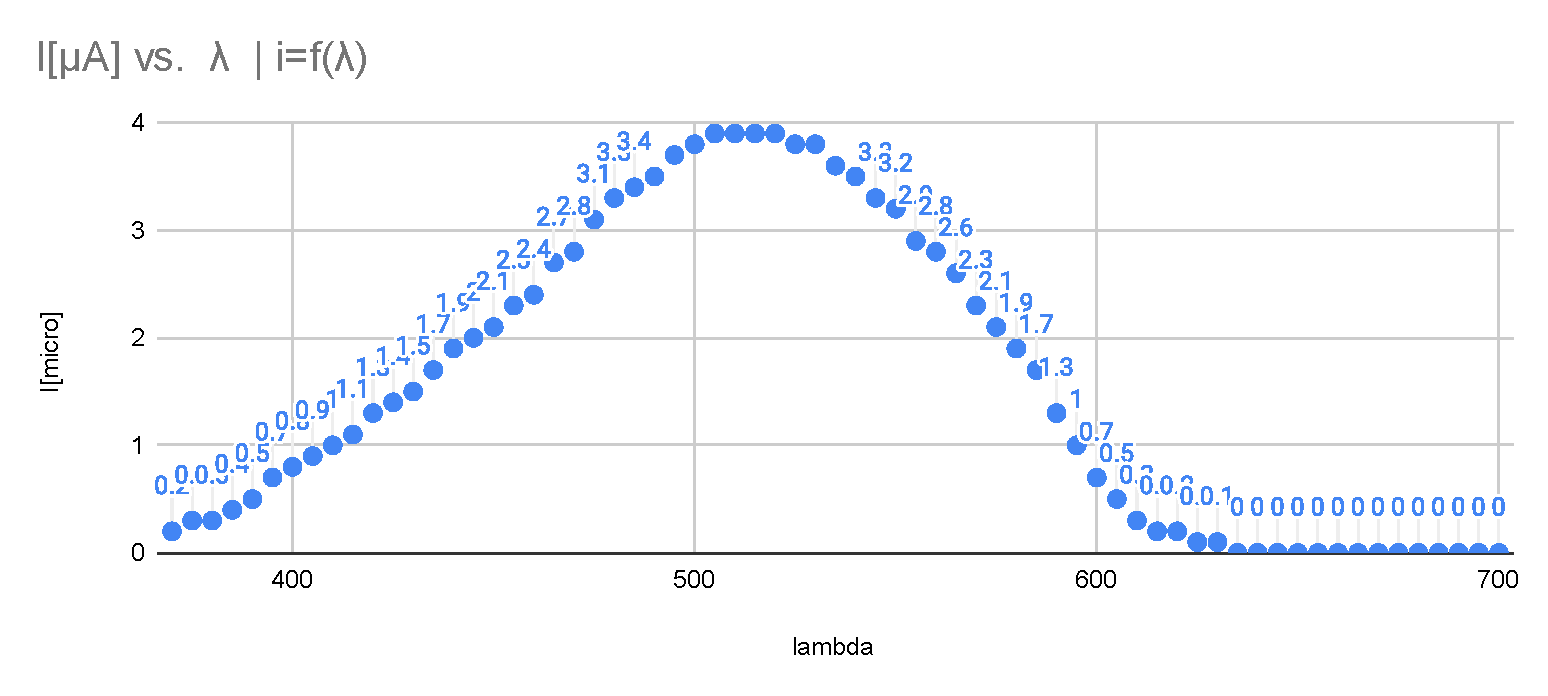
\includegraphics[width=10cm]{schematics/thresholdWavelenght.pdf}
	\caption{Estimating the value of the treshold wavelength}
\end{figure}

\begin{figure}[H]
	\centering
	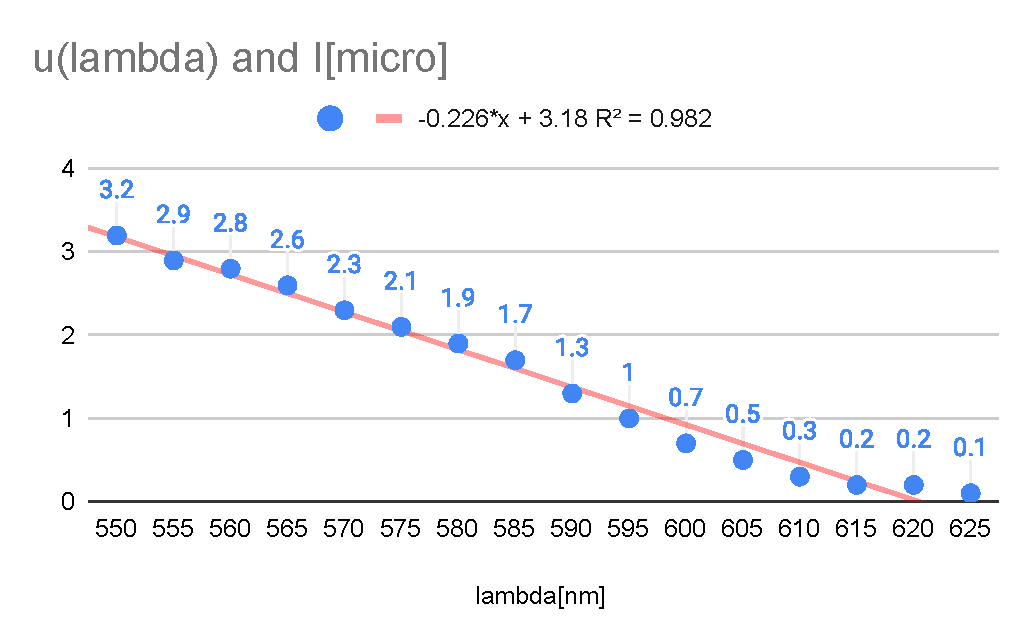
\includegraphics[width=10cm]{schematics/spectralCharacteristic.pdf}
	\caption{Approximate the long-wave edge of the spectral characteristic}
\end{figure}

\begin{table}[H]
    \centering
    \begin{tabular}{l|l|l|l|l|l}
        a & u(a) & b & u(b) & $\lambda_o nm$ & $u_c(\lambda_o) nm$ \\ \hline
        -0.226 & 0.0019 & 140 & 1.1 & 619.5 & 7.1 \\ 
    \end{tabular}
\end{table}

\subsubsection*{Calculations }

\begin{equation}
	\lambda_o = - \frac{b}{a} = -\frac{140}{-0.226} = 6.19.5 nm
\end{equation}
\begin{equation}
	u_c(\lambda_0)=\sqrt{(-\frac1a \cdot u(b))^2 + (\frac{b}{a^2} \cdot u(a))^2} \approx 7.1nm
\end{equation}

\begin{table}[H]
    \centering
    \begin{tabular}{l|l|l|l|l|l}

        $\lambda_0$ [nm] & u($\lambda_0$) [nm] & W [J] & $u_c$(W) [J] & $E_k$max [J] & uc(Ekmax)[J] \\ \hline
        619.5 & 7.1 & 3.21E-19 & 0 & -3.20E-19 & 0 \\ 
    \end{tabular}
\end{table}

\subsubsection*{Calculations }

\begin{equation}
	W = \frac{h\cdot c}{\lambda_0} = \SI{3.21E-19 }{\joule}
\end{equation}






\subsection{Measurements of current-voltage characteristics}

In this exercise are going to take measurements of the current-voltage characteristics.
Measure the current-voltage characteristics of the photocell.

\begin{table}[H]
    \centering
    \begin{tabular}{l|l|l|l}

        V [V] & u(U) [V] & I [\SI{}{\micro\ampere}] & u(I) [\SI{}{\micro\ampere}] \\ \hline
        0.2 & 0.00106 & 0.1 & 0.019 \\ \hline
        1.4 & 0.00729 & 0.8 & 0.024 \\ \hline
        2.2 & 0.01145 & 1.1 & 0.027 \\ \hline
        3.1 & 0.01612 & 1.6 & 0.031 \\ \hline
        4 & 0.0208 & 1.9 & 0.033 \\ \hline
        5 & 0.026 & 2.2 & 0.036 \\ \hline
        6 & 0.03119 & 2.5 & 0.038 \\ \hline
        7 & 0.03639 & 2.7 & 0.04 \\ \hline
        8.3 & 0.04314 & 3 & 0.042 \\ \hline
        9 & 0.04678 & 3.1 & 0.043 \\ \hline
        10.3 & 0.05354 & 3.3 & 0.044 \\ \hline
        12 & 0.06237 & 3.5 & 0.046 \\ \hline
        14.4 & 0.07484 & 3.7 & 0.048 \\ \hline
        16 & 0.08315 & 3.7 & 0.048 \\ \hline
        18 & 0.09355 & 3.7 & 0.048 \\ \hline
        20.2 & 0.10498 & 3.7 & 0.048 \\ \hline
        22 & 0.11433 & 3.7 & 0.048 \\ \hline
        24.1 & 0.12524 & 3.7 & 0.048 \\ \hline
        26 & 0.13512 & 3.7 & 0.048 \\ \hline
        28 & 0.14551 & 3.7 & 0.048 \\ \hline
        30.1 & 0.15642 & 3.7 & 0.048 \\ \hline
        40.1 & 0.20838 & 3.7 & 0.048 \\ \hline
        50.2 & 0.26086 & 3.7 & 0.048 \\ \hline
        60 & 0.31179 & 3.7 & 0.048 \\ \hline
        70 & 0.36375 & 3.7 & 0.048 \\ \hline
        80 & 0.41571 & 3.7 & 0.048 \\ \hline
        90 & 0.46767 & 3.7 & 0.048 \\ \hline
        100 & 0.51963 & 3.7 & 0.048 \\ \hline
        110 & 0.57159 & 3.7 & 0.048 \\ \hline
        115 & 0.59757 & 3.7 & 0.048 \\ 
    \end{tabular}
    \caption{$\lambda = 520 nm $}
\end{table}


\begin{figure}[H]
	\centering
	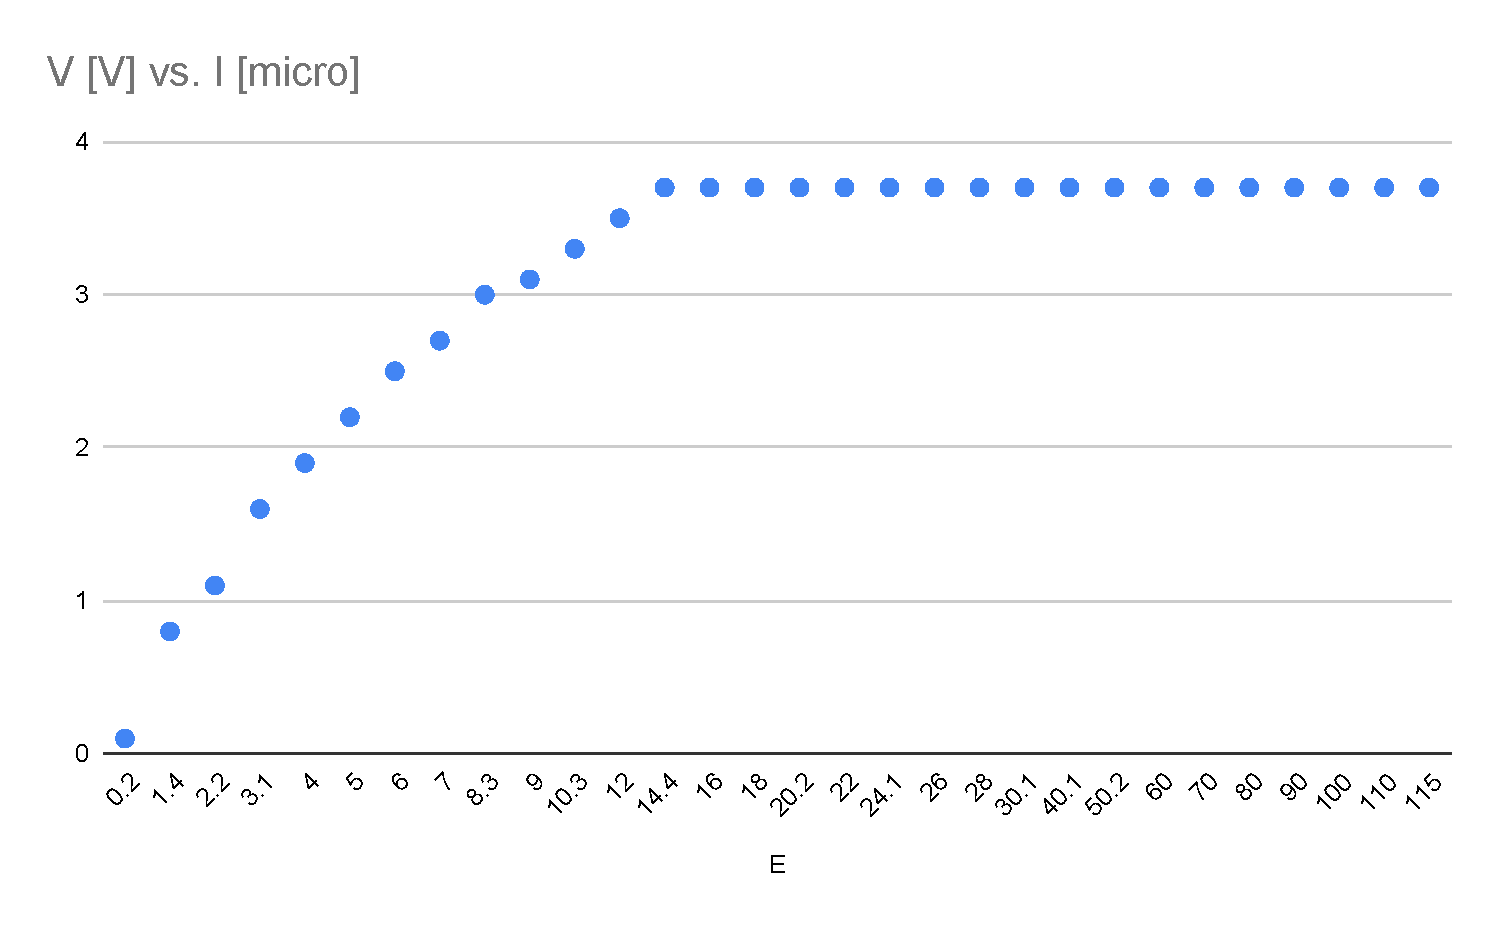
\includegraphics[width=10cm]{schematics/currentVoltageCharacteristics.pdf}
	\caption{Light intensities used in the experiment}
\end{figure}

\begin{table}[H]
    \centering
    \begin{tabular}{l|l}
    
        Is [\SI{}{\micro\ampere}] & u(Is) [\SI{}{\micro\ampere}] \\ \hline
        3.700 & 0.048 \\ 
    \end{tabular}
    \caption{Estimated current saturation. (We assume that is
is the value of current at the polarization of approximately 115V).}
\end{table}

In our exercise, the graph made of our measurements is similar to the graph we have found in instruction, so we can assume that our measurements were made correctly.




